
\documentclass[titlepage = firstcover]{scrartcl}
\usepackage[aux]{rerunfilecheck}
\usepackage{fontspec}
\usepackage[main=ngerman, english, french]{babel}

% mehr Pakete hier
\usepackage{expl3}
\usepackage{xparse}

%Mathematik------------------------------------------------------
\usepackage{amsmath}   % unverzichtbare Mathe-Befehle
\usepackage{amssymb}   % viele Mathe-Symbole
\usepackage{mathtools} % Erweiterungen für amsmath
\usepackage{dsfont}
\usepackage[
  math-style=ISO,    % \
  bold-style=ISO,    % |
  sans-style=italic, % | ISO-Standard folgen
  nabla=upright,     % |
  partial=upright,   % /
]{unicode-math}% "Does exactly what it says on the tin."
\usepackage[section, below]{placeins}

% Laden von OTF-Mathefonts
% Ermöglich Unicode Eingabe von Zeichen: α statt \alpha

\setmathfont{Latin Modern Math}
%\setmathfont{Tex Gyre Pagella Math} % alternativ zu Latin Modern Math
\setmathfont{XITS Math}[range={scr, bfscr}]
\setmathfont{XITS Math}[range={cal, bfcal}, StylisticSet=1]

\AtBeginDocument{ % wird bei \begin{document}
  % werden sonst wieder von unicode-math überschrieben
  \RenewDocumentCommand \Re {} {\operatorname{Re}}
  \RenewDocumentCommand \Im {} {\operatorname{Im}}
}
\usepackage{mleftright}
\setlength{\delimitershortfall}{-1sp}
\usepackage[version=4]{mhchem}

%Sprache----------------------------------------------------------
\usepackage{microtype}
\usepackage{xfrac}
\usepackage[autostyle]{csquotes}    % babel
\usepackage[german, unicode, pdfusetitle]{hyperref}
\usepackage{bookmark}
\usepackage[shortcuts]{extdash}
%Einstellungen hier, z.B. Fonts
\usepackage{booktabs} % Tabellen

\setlength{\parindent}{0pt}

\title{V406 - Beugung am Spalt}
\author{
  David Gutnikov\\
  \href{mailto:david.gutnikov@udo.edu}{david.gutnikov@udo.edu}\\
  Lasse Sternemann\\
  \href{mailto:lasse.sternemann@udo.edu}{lasse.sternemann@udo.edu}
}
\date{Bearbeitet am 23.06.2020}

\begin{document}
    \maketitle
    \newpage
    \tableofcontents
    \newpage

    \section{Theorie}
        Das Phänomen der Beugung von Licht tritt auf, wenn Licht auf Objekte oder Spalte trifft, deren Ausmaße klein gegen die des einfallenden Lichtstrahls sind. Die zugehörige physikalische
        Beschreibung ist nicht mit der Beschreibung von Licht als Quantenobjekt möglich. Stattdessen wird auf den Wellencharakter des Lichts zurückgegriffen, der es ermöglicht das Huygensche
        Prinzip zu nutzen. Dieses beruht darauf, dass eine Wellenfront aus vielen Elementarwelle besteht. Wenn die Wellenfront auf ein Hindernis trifft, laufen nur einzelne Elemtarwellen weiter,
        die untereinander interferieren und so die Beugung erklären.

        \subsection{Näherungen zur Untersuchung von Beugung am Einzelspalt}
            Die Beugung von Licht an einem einzelnen Spalt kann über zwei Näherungen beschrieben werden, die sich hinsichtlich
            \FloatBarrier

            \begin{figure}[h]
              \centering
              \includegraphics[width = 0.8\textwidth]{Bilder/Näherungen.png}
              \caption{In der Abbildung ist auf der linken Seite die Fresnel-Näherung zu sehen und auf der rechten Seite die Fraunhofer-Näherung, bei der eine ebene einfallende Wellenfront angenommen wird und somit die Rechnung stark vereinfacht wird. [1]}
              \label{fig:Näherungen}
            \end{figure}

            \FloatBarrier

            \noindent
            \subsubsection*{Fresnel-Näherung}
                Bei der Fresnel-Näherung ist der Abstand zwischen Lichtquelle, Spalt und Schirm endlich. Daher ist der einfallende Strahl nicht parallel, sondern läuft, wie in Abbildung 
                \ref{fig:Näherungen} a) zu sehen auseinander. Daher werden Strahlen, die auf dem Schirm miteinander interferieren, am Spalt nicht im gleichem Winkel gebeugt.

            \subsubsection*{Fraunhofer-Näherung}
                Die in Abbildung \ref{fig:Näherungen} b) zu sehende Fraunhofer beruht darauf, dass die Lichtquelle ins Unendliche von Spalt und Schrim entfernt wird, sodass der einfallende 
                Lichtstrahl als parallel angenommen werden kann. Nun werden zwei interferierende Strahlen im selben Winkel gebeugt. Zusätzlich werden die gebeugten Strahlen durch eine 
                Sammellinse auf den Schirm projeziert, sodass auch der Schrim quasi unendlich weit entfernt vom SPalt ist und somit die zweite Bedingung für die Fraunhofer-Näherung erfüllt ist.
                Da der gemeinsamme Beugungswinkel die Rechnung immens vereinfacht, wird für den Versuch die Fraunhofer-Näherung erfüllt.
                
    
        \subsection{Mathematische Beschreibung der Beugung am Einzelspalt}
            Bei der Beschreibung der Beugung am Einzelspalt wird von einer unendlichen Entfernung zwischen Quelle, Spalt und Schirm ausgegangen, sodass die Fraunhofer-Näherung angewandt werden kann.
            Dementsprechen trifft eine parallele Wellenfront auf den Spalt. Diese kann über folgende Formel als ebene Welle beschrieben werden, die in z-Richtung läuft:

            \begin{equation*}
                A(z,t) = \text{A}_0 \cdot e^{i\left(\omega t - \frac{2\pi z}{\lambda}\right)}
            \end{equation*}

            \noindent
            Dabei bezeichnet $\omega$ die Frequenz des Lichts, $\text{A}_0$ die Amplitude des Lichts und $\lambda$ dessen Wellenlänge. \newline
            
            \FloatBarrier

            \begin{figure}[h]
              \centering
              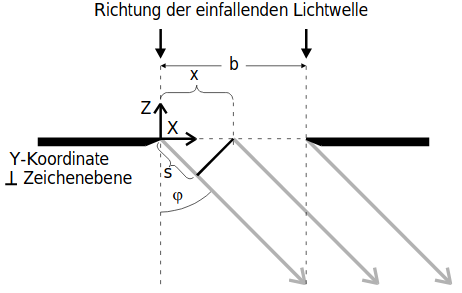
\includegraphics[width = 0.6\textwidth]{Bilder/Phasendifferenz.png}
              \caption{In der Abbildung ist Entstehung der Phasendifferenz zwischen zwei Strahlen, die unter dem selben Winkel $\varphi$ gebeugt werden, dargestellt. [1]}
              \label{fig:Phasendifferenz}
            \end{figure}

            \FloatBarrier

            \noindent

            Wie bereits beschrieben entstehen beim Auftreffen der ebenen Welle auf den Spalt viele neue elementare Kugelwellen. In Abhängigkeit vom Beugungswinkel weisen diese einen Phasenunterschied
            auf. Dies lässt sich bildlich in Abbildung \ref{fig:Phasendifferenz} nachvollziehen. Bis die mittlere Kugelwelle entsteht, hat sich die, in einem Abstand x entfernte Kugelwelle, bereits 
            eine gewisse Zeit und demnach Distanz s ausgebreitet. Die beiden Strahlenbündel weisen daher folgenden Phasenunterschied auf:

            \begin{equation}
                \delta = \frac{2\pi \text{s}}{\lambda} = \frac{2\pi \text{x} \sin(\varphi)}{\lambda}
                \label{eqn:Phasendiff}
            \end{equation}

            \noindent
            Um die resultierende Welleenamplitude unter dem Winkel $\varphi$ zu bestimmen müssen alle unter dem Winkel vom Spalt auslaufenden Strahlenbündel summiert werden. Das Verringern der 
            Distanz x zwischen den Strahlenbündeln auf ein Infinuum wandelt die Summe in folgendes Integral über die Spalbreite b um, das die Amplitude B unter Berücksichtigung des Phasenunterschieds 
            zwischen den auslaufenden Strahlenbündeln in Abhängigkeit von der Distanz zum Spalt z, der Zeit t und dem Winkel $\varphi$ angibt.

            \begin{align}
                B(z, t, \varphi) &= \text{A}_0 \cdot \int_0^b e^{i\left(\omega t - \frac{2 \pi z}{\lambda + \delta}\right)} \, dx = \text{A}_0 \cdot e^{i\left(\omega t - \frac{2 \pi z}{\lambda}\right)} \int_0^b e^{\left(\frac{2\pi i \text{x} \sin(\varphi)}{\lambda}\right)} \, dx \\
                B(z, t, \varphi) &= \text{A}_0 \cdot e^{i\left(\omega t - \frac{2 \pi z}{\lambda}\right)} \cdot e^{\frac{i \pi \text{b} \sin(\varphi)}{\lambda}} \cdot \frac{\lambda}{\pi \sin(\varphi)} \cdot \sin \left(\frac{\pi \text{b} \sin (\varphi)}{\lambda}\right)
                \label{eqn:BEinzel}
            \end{align}

            \noindent
            Der für die Abhängigkeit vom Winkel $\varphi$ entscheidende Part ist unabhhängig von den zwei Exponentialfunktionen, sodass Gleichung \ref{eqn:BEinzel} für die Untersuchung der 
            Intensitätsverteilung in Abhängigkeit vom Winkel in folgende Form umgeschrieben werden kann.

            \begin{equation}
                B(\varphi) = \text{A}_0 \text{b} \cdot \frac{\sin(\eta)}{\eta} \qquad \text{mit} \qquad \eta := \frac{\pi \text{b} \sin (\varphi)}{\lambda}
                \label{eqn:Winkelabhängigkeit}
            \end{equation}

            \noindent
            Die Funktion hat folgende periodische Nulstellen
            
            \begin{equation}
                \sin(\varphi) = \pm \text{n} \cdot \frac{\lambda}{\text{b}} \, , \text{n} \in \mathds{Z}
                \label{eqn:NSTEinzel}
            \end{equation}

            \noindent
            und ist Abbildung \ref{fig:BEinzel} dargestellt.

            \FloatBarrier

            \begin{figure}[h]
              \centering
              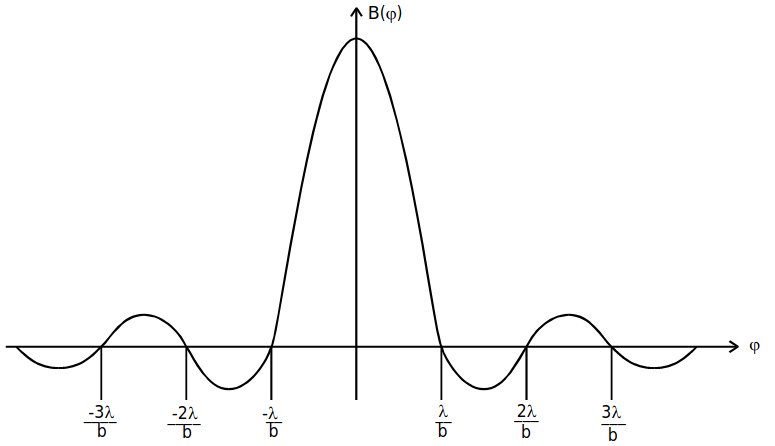
\includegraphics[width = 0.7\textwidth]{Bilder/BEinzel.png}
              \caption{In der Grafik ist die Intensitätsverteilung der gebeugten Strahlung in Abhängigkeit vom Beugungswinkel $\varphi$ dargestellt. Im Experiment wird das Hauptmaximum und die beiden ersten Nebenmaxima bei $\pm \frac{\lambda}{b}$ untersucht. [1]}
              \label{fig:BEinzel}
            \end{figure}

            \FloatBarrier

            \noindent

            Die experimentelle Beobachtung des Lichts findet wie üblich über die Messung der Intensität statt. Diese ist das Quadrat der Amplitude, sodass folgender Zusammenhang gilt.

            \begin{equation}
                I(\varphi) \propto B(\varphi)^2 = \text{A}_0^2 \text{b}^2 \cdot \left(\frac{\lambda}{\pi \text{b} \sin(\varphi)}\right)^2 \cdot \sin^2 \left(\frac{\pi \text{b} \sin(\varphi)}{\lambda}\right)
                \label{eqn:IEinzel}
            \end{equation}


            \newpage
            \subsection{Mathematische Beschreibung der Beugung am Doppelspalt}
                \FloatBarrier

                \begin{figure}[h]
                  \centering
                  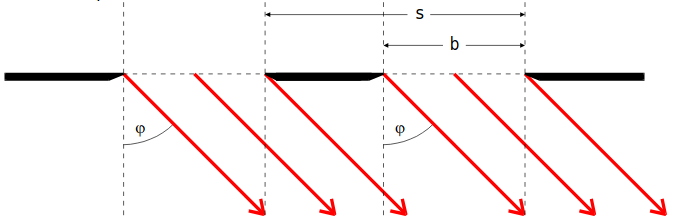
\includegraphics[width = 0.6\textwidth]{Bilder/Doppelspalt.png}
                  \caption{In der Abbildung ist der Fall eines Doppelspalts schematisch dargestellt. Die eingzeichneten Strahlen treten im selben Winkel aus dem jeweiligen Spalt aus. S beschreibt die Distanz vom Mittelpunkt eines Spalts zum Nächsten. Diese haben eine Breite b. [1]}
                  \label{fig:Doppelspalt}
                \end{figure}
            
                \FloatBarrier
            
                \noindent
                \subsubsection*{Überlagerung zweier Einzelspalte}
                    Die intuitive Methode das Beugungsverhalten eines Doppelspalts zu beschreiben, ist die Überlagerung der Beugungsverteilung zweier Einzelspalte. Unter Annahme der Fraunhofer-
                    Näherung ändert sich das Beugungsverhalten im Vergleich zum Einzelspalt einzig durch das Hinzukommen eines Cosinus-quadrat-Faktors und es ergibt sich folgende 
                    Intensitätsverteilung.

                    \begin{equation}
                        I(\varphi) \propto B(\varphi)^2 = 4 \cdot \cos^2\left(\frac{\pi \text{s} \sin \varphi}{\lambda}\right) \cdot \left(\frac{\lambda}{\pi \text{b} \sin(\varphi)}\right)^2 \cdot \sin^2 \left(\frac{\pi \text{b} \sin(\varphi)}{\lambda}\right)
                        \label{eqn:IDoppel}
                    \end{equation}

                    \noindent
                    Diese Intensitätsverteilung besitzt Minima 1-ter Ordnung, die den Nulstellen der Amplitudenfunktion \ref{eqn:BEinzel} des Einzelspalts entsprechen und zusätzlich noch Minima bei
                    den Nullstellen des Cosinus-quadrat-Faktors:

                    \begin{equation}
                        \varphi(\text{k}) = \arcsin \left(\frac{2\text{k} + 1}{2\text{s}}\right) \cdot \lambda \, , \text{k} \in \mathds{Z}
                        \label{eqn:NSTCOShoch2}
                    \end{equation}


                \subsubsection*{Fouriertransformation der Aperturfunktion}
                    Neben der Bestimmung per Überlagerung zweier Einzelspaltverteilungen, lässt sich die Amplitudenverteilung auch über die Fouriertransformation der Aperturfunktion berechnen. Die
                    Aperturfunktion beschreibt dabei das Beugungsobjekt. Eine unendliche Wand mit einem Spalt der Breite B hat somit folgende Aperturfunktion, da nur am Spalt Licht durch die
                    Wand dringen kann.

                    \begin{equation*}
                        f(x) =  \begin{cases}
                            \text{A}_0 \qquad \text{für} \qquad 0 \leqslant x \leqslant b \\
                            0 \qquad \qquad \: \: \text{sonst}
                        \end{cases}
                    \end{equation*}

                    \noindent
                    Die Fouriertransformation dieser Aperturfunktion liefert folgende Amplitudenfunktion

                    \begin{equation}
                        g(\zeta) := \int_{-\infty}^{+\infty} f(x) \cdot e^{ix\zeta} dx = \text{A}_0 \int_0^{\text{b}} e^{ix\zeta} dx = \frac{2\text{A}_0}{\zeta} \cdot e^{\left(\frac{i\zeta \text{b}}{2}\right)} \cdot \sin\left(\frac{\zeta\text{b}}{2}\right)
                        \label{eqn:AmplitudeFT}
                    \end{equation}

                    \noindent
                    mit $\zeta := \frac{2\pi \sin(\varphi)}{\lambda}$. Dies entspricht der bereits bestimmten Amplitudenverteilung eines Einzelspalts. Nun kann die Aperturfunktion einfach auf
                    einen Doppelspalt ausgeweitet werden. Dies kann dann zum Beispiel so aussehen, sofern der Abstand der beiden Spalte geringer ist, als die Breite des Strahls:

                    \begin{equation*}
                        f(x) =  \begin{cases}
                            \text{A}_0 \qquad \text{für} \qquad 0 \leqslant x \leqslant b \\
                            \text{A}_0 \qquad \text{für} \qquad c \leqslant x \leqslant d \\
                            0 \qquad \qquad \: \: \text{sonst}
                        \end{cases}
                    \end{equation*}

                    \noindent
                    mit $ b < c < d$. Ein großer Vorteil besteht darin, dass die Fouriertransformation umkehrbar ist und die Aperturfunktion demnach die Fouriertransformierte der Amplitudenverteilung
                    ist. So lassen sich aus der Bestimmung der Amplitudenverteilung die Aperturfunktion und somit die Eigenschaften des Beugungsobjekts bestimmen.

    
    \newpage
    \section{Aufbau und Durchführung}
        \subsection{Aufbau}
            \FloatBarrier

            \begin{figure}[h]
              \centering
              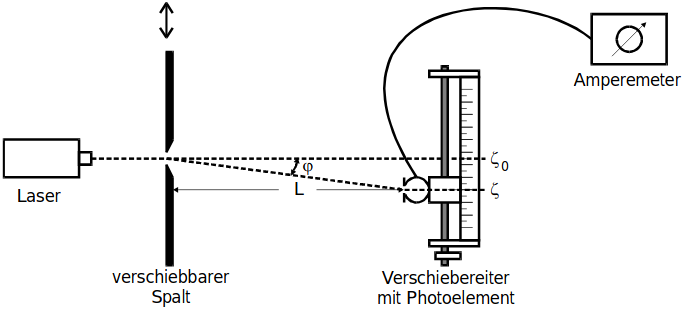
\includegraphics[width = 0.6\textwidth]{Bilder/Aufbau.png}
              \caption{In der Abbildung ist der Aufbau zur Untersuchung des Beugungsverhalten zu sehen. Der Laser strahlt auf den Schirm, in dessen Mitte sich ein Einzelspalt findet. In fester Entfernung befindet sich ein Photostrommessgerät auf einem Schieberegler, der auf einer Skala relativ zum Mittelpunkt des Strahls verschoben werden kann. [1]}
              \label{fig:Aufbau}
            \end{figure}
        
            \FloatBarrier
        
            \noindent

            Wie in Abbildung \ref{fig:Aufbau} zu sehen leuchtet ein Laser mit monochromatischem Licht auf eine Wand. Dort wo der Strahl auftrifft, können verschiedene Blenden aufgesetzt werden. Diese
            ermöglichen das einfache Wechseln von der Bestrahlung eines Einzelspalts, Doppelspalts oder auch Gitter. In einer konstanten Entfernung L=116,2 cm befindet sich eine Photodiode, die in der Lage
            ist die einfallende Intensität über einen Photostrom zu messen. Zudem ist sie auf einer Skala befestigt, die die Positionierung der Photodiode in Relation zum Zentrum des Laserstrahls
            angibt.
            
        \subsection{Durchführung}
            Aufgrund mangelnder Zeit wird nur das Beugungsbild eines Einzelspalts untersucht.
            \subsubsection*{Untersuchung eines Einzelspalts}
                Zur Untersuchung des Einzelspalts wird eine Blende in der Wand befestigt, die einen einzelnen Spalt mit der Breite 0,15 mm enthält. Dieser wird im Zentrum des
                Laserstrahls positioniert, sodass eine ebene Welle auf ihn trifft. Nun wird das Hauptmaximum in Abständen von 0,3 mm, sowie die beiden ersten Nebenmaxima in Abständen von 0,5 mm 
                vermessen. Zusätzlich muss eine Nullmessung des Photostroms durchgeführt werden, um im Nachhinein den Untergrund durch ungewollte Lichtquellen abziehen zu können. 


    \newpage
    \section{Auswertung}
        Zuerst wurde der Dunkelstrom, d.h. der durch das natürlich vorhandene Licht ausgelöste Strom, gemessen.
        Für diesen wurde aufgrund des stark abgedunkelten Zimmers ein Strom von $(1 \pm 0,2)$ nA gemessen.
        Dieser Wert ist um eine bis zwei Zehnerpotenzen kleiner als die Messunsicherheiten der Messwerte für den Strom bei eingeschaltetem Laser.
        Deswegen würde den Dunkelstrom von den Messwerten abzuziehen die Messergebnisse nicht beeinflussen.

        \begin{figure}[h]
            \centering
            \includegraphics[width = 0.8\textwidth]{Bilder/Einzelspalt_Messwerte.png}
            \caption{Hier ist der Strom gegen den Winkel $\phi$ aus \autoref{fig:Phasendifferenz} aufgetragen. Die Messwerte dafür befinden sich in \autoref{tab:Messwerte}}
            \label{fig:Einzelspalt_Messwerte}
        \end{figure}

        \FloatBarrier

        Es wird eine Ausgleichsrechnung durchgeführt, wobei der Sinus cardinalis \\ $\text{sinc}(x) = \sin(x) / x$ an die Messwerte gefittet wird. Dazu wird \autoref{eqn:IEinzel} verwendet und ein Faktor $k$ für die Proportionalität zwischen $B(\varphi)$ und $I(\varphi)$ eingeführt. Um Größen zu erhalten, mit denen der Computer besser rechnen kann wird von folgenden Substitutionen Gebrauch gemacht,
        \begin{equation*}
            I_0 = k \cdot A_0^2 \cdot b^2 \qquad \text{und} \qquad \xi = \frac{b}{\lambda}
        \end{equation*}
        sodass \autoref{eqn:BEinzel} mit ihnen aussieht wie:
        \begin{equation*}
            I(\varphi) = I_0 \cdot \text{sinc}\bigl(\xi \cdot \sin(\varphi)\bigr)
        \end{equation*}

        Es ergeben sich für die beiden Parameter $I_0 = 3,24 \pm 0,02$ und $240.1 \pm 2,6$. Mit der Wellenlänge des Lasers $\lambda = 633\,$nm ist dann $b = 0,152\,$mm. Dieser Wert weicht um $a_b = 1,3\,$\% vom Literaturwert $b_{\text{lit}} = 0,15\,$mm ab. 


        \newpage
        \section{Diskussion}
            Wir konnten leider wegen dem Zeitmangel keine Werte für den Doppelspalt aufnehmen und mussten uns mit den Messwerten zum Einzelspalt begnügen.

            Da die Schrittweite vergleichsweise klein war und das Hauptmaximum mit einer noch kleineren Schrittweit durchmessen wurde, liegt die theoretische Kurve sehr nah an den Messwerten und ermöglicht eine genaue Bestimmung der Spaltbreite. Diese weicht nur um ca. $1,3\,$\% vom Literaturwert ab.

            Hinzu kommt auch, dass der Raum in dem der Versuch durchgeführt wurde sehr stark abgedunkelt war, sodass fast kein natürliches Licht an den Detektor kam. Deswegen war der Dunkelstrom so gering, dass er die Messwerte nicht beeinflusst hat.


    \newpage
    \section{Daten}
        \begin{table}[h]
            \centering
            \caption{Hier sind die Abstände vom Hauptmaximum $a$, der Winkel $\phi$ zwischen der Strecke vom Einzelspalt und einem Punkt auf dem Schirm, der gemessene Strom $I$ und seine Messunsucherheit $I_{\text{u}}$ dargestellt.}
            \label{tab:Messwerte}
            \begin{tabular}{c c c c | c c c c}
                \toprule
                {$a$ [mm]} & {$\phi$ [°]} & {$I$ [$\mu$A]} & {$I_{\text{u}}$ [$\mu$A]} & {$a$ [mm]} & {$\phi$ [°]} & {$I$ [$\mu$A]} & {$I_{\text{u}}$ [$\mu$A]} \\
                \midrule
                -9.00   &  -0.44   &   0.10   &   0.02   &    0.30   &   0.01   &  10.80   &   0.20 \\
                -8.50   &  -0.42   &   0.20   &   0.02   &    0.60   &   0.03   &  10.80   &   0.20 \\
                -8.00   &  -0.39   &   0.32   &   0.02   &    0.90   &   0.04   &   9.60   &   0.20 \\
                -7.50   &  -0.37   &   0.44   &   0.02   &    1.20   &   0.06   &   9.00   &   0.20 \\
                -7.00   &  -0.35   &   0.48   &   0.02   &    1.50   &   0.07   &   7.80   &   0.20 \\
                -6.50   &  -0.32   &   0.42   &   0.02   &    1.80   &   0.09   &   6.60   &   0.20 \\
                -6.00   &  -0.30   &   0.30   &   0.02   &    2.10   &   0.10   &   5.40   &   0.20 \\
                -5.50   &  -0.27   &   0.16   &   0.02   &    2.40   &   0.12   &   4.20   &   0.20 \\
                -5.00   &  -0.25   &   0.08   &   0.02   &    2.70   &   0.13   &   3.60   &   0.20 \\
                -4.50   &  -0.22   &   0.16   &   0.02   &    3.00   &   0.15   &   2.60   &   0.20 \\
                -4.20   &  -0.21   &   0.36   &   0.02   &    3.30   &   0.16   &   1.80   &   0.20 \\
                -3.90   &  -0.19   &   0.68   &   0.02   &    3.60   &   0.18   &   1.00   &   0.20 \\
                -3.60   &  -0.18   &   1.00   &   0.20   &    3.90   &   0.19   &   0.66   &   0.02 \\
                -3.30   &  -0.16   &   1.60   &   0.20   &    4.20   &   0.21   &   0.32   &   0.02 \\
                -3.00   &  -0.15   &   2.40   &   0.20   &    4.50   &   0.22   &   0.16   &   0.02 \\
                -2.70   &  -0.13   &   3.20   &   0.20   &    5.00   &   0.25   &   0.10   &   0.02 \\
                -2.40   &  -0.12   &   4.20   &   0.20   &    5.50   &   0.27   &   0.24   &   0.02 \\
                -2.10   &  -0.10   &   5.20   &   0.20   &    6.00   &   0.30   &   0.42   &   0.02 \\
                -1.80   &  -0.09   &   6.20   &   0.20   &    6.50   &   0.32   &   0.58   &   0.02 \\
                -1.50   &  -0.07   &   7.20   &   0.20   &    7.00   &   0.35   &   0.62   &   0.02 \\
                -1.20   &  -0.06   &   8.00   &   0.20   &    7.50   &   0.37   &   0.58   &   0.02 \\
                -0.90   &  -0.04   &   8.80   &   0.20   &    8.00   &   0.39   &   0.46   &   0.02 \\
                -0.60   &  -0.03   &   9.40   &   0.20   &    8.50   &   0.42   &   0.30   &   0.02 \\
                -0.30   &  -0.01   &   9.60   &   0.20   &    9.00   &   0.44   &   0.18   &   0.02 \\
                 0.00   &   0.00   &  11.40   &   0.20 \\
                \bottomrule
            \end{tabular}
        \end{table}
  
      \FloatBarrier
    
    \newpage
    \section{Literatur}
        [1] \textit{Versuchsanleitung V406 - Beugung am Spalt.} TU Dortmund, 2020 \newline

\end{document}

        